\documentclass[a4paper]{scrreprt}

\usepackage[ngerman]{babel}
\usepackage[utf8]{inputenc}
\usepackage[T1]{fontenc}
\usepackage{ae}
\usepackage[bookmarks,bookmarksnumbered]{hyperref}
\usepackage{tabularx}
\usepackage{graphicx}
\usepackage[german]{fancyref}
\usepackage[
nonumberlist,
toc,
section]
{glossaries}

\makeglossaries
\newglossaryentry{Produkt}
{
name={Produkt},
plural={Produkte},
description={ das von uns gelieferte Softwaresystem}
}
\newglossaryentry{Webbrowser}
{
name={Webbrowser},
plural={Webbrowser},
description={Für dieses Produkt wird nur auf Google Chrome und Mozilla Firefox hin entwickelt.}
}
\newglossaryentry{Spiel}
{
name={Spiel},
plural={Spiele},
description={Ein Spiel ist eine Instanz eines \Gls{Spielmodus}. Ein Spiel hat das Ziel das Wissen des Spielers zu nutzen um die Merkmalsauswahl für Machine Learning zu unterstützen.}
}
\newglossaryentry{Spielmodus}
{
name={Spielmodus},
plural={Spielmodi},
description={Ein Spielmodus ist eine definierte Art und Weise, die Merkmalsauswahl durchzuführen. Standardmäßig gibt es die Spielmodi \Gls{Matrix Select} und \Gls{Binär Select}.}
}
\newglossaryentry{Matrix Select}
{
name={Matrix Select},
plural={Matrix Select},
description={Matrix Select ist ein \Gls{Spielmodus}, in dem ein \Gls{Spieler} aus einer bestimmten Anzahl an Merkmalen eine Teilmenge auswählt.}
}
\newglossaryentry{Binär Select}
{
name={Binär Select},
plural={Binär Select},
description={Binär Select ist ein \Gls{Spielmodus}, in dem ein \Gls{Spieler} Merkmale jeweils paarweise vergleicht und eins auswählt.}
}
\newglossaryentry{Spieler}
{
name={Spieler},
plural={Spieler},
description={Ein Spieler ist ein Nutzer, welcher an einem Spiel teilnehmen kann. Meist ist dies ein Angestellter des Betriebs.}
}
\newglossaryentry{Spieleinstellungen}
{
name={Spieleinstellungen},
plural={Spieleinstellungen},
description={Einstellungen für ein Spiel umfassen: die Merkmale welche ausgewählt werden soll, die Art des Spiels, die teilnehmenden Spieler, Endbedingungen des Spiels}
}
\newglossaryentry{Organisator}
{
name={Organisator},
plural={Organisatoren},
description={Ein Organisator ist ein Nutzer, der neue Spiele erstellt und die Ergebnisse von diesen ausliest.}
}
\newglossaryentry{Achievement}
{
name={Achievement},
plural={Achievements},
description={Ein Ziel oder eine Errungenschaft, welche den Spieler motiviert weiter zu spielen.}
}
\newglossaryentry{Administrator}
{
name={Administrator},
plural={Administratoren},
description={Die Person, welche das System installiert und den Nutzern zur Verfügung stellt. Sie verwaltet den
\Gls{Spiele-Server}}
}
\newglossaryentry{Spiele-Server}
{
name={Spiele-Server},
plural={Spiele-Server},
description={Ein Computer, der der Verwaltung von CS:Select dient und Internetanbindung hat.}
}

\begin{document}

    \title{Pflichtenheft CS-Select}
    \author{PSEArmee}
    \maketitle

    % Platzierung des Inhaltsverzeichnisses
    \tableofcontents

    \chapter{Zielbestimmung}
    Eine Organisation soll durch das \Gls{Produkt} das Domänenwissen ihrer Mitarbeiter dazu nutzen die Merksmalsauswahl für ein Machine-Learning-Modell zu vereinfachen.

    \section{Musskriterien}
    \begin{tabular}{ l | l}
        /FA10/ & Ein \Gls{Spieler} muss sich anmelden können. \\
        /FA20/ & Ein \Gls{Spieler} muss sich registrieren können. \\
        /FA30/ & Ein \Gls{Organisator} muss sich anmelden können. \\
        /FA40/ & Ein \Gls{Organisator} muss ein \Gls{Spiel} erstellen und beenden können. \\
        /FA50/ & Die Anmeldung muss in einem modernem \Gls{Webbrowser} möglich sein. \\
        /FA60/ & \Gls{Spieler} müssen bei einem \Gls{Spiel} mitspielen können. \\
        /FA70/ & Ein \Gls{Organisator} muss \Gls{Spieler} zu einem \Gls{Spiel} einladen können. \\
        /FA80/ & Die Ergebnisse eines \Gls{Spiel} können ausgelesen werden. \\
        /FA90/ & Ein Spiel muss Endbedingungen besitzen. \\
        /FA100/ & Ein Spiel muss bei Erreichen seiner Endbedingungen enden. \\
        /FA110/ & Das System muss mit dem ML-Server kommunizieren. \\
        /FA120/ & Der Organisator kann in einem GUI den Spielstand überprüfen.\\
    \end{tabular}

    \section{Kannkriterien}
    \begin{tabularx}{\linewidth}{@{}>{\bfseries}l@{\hspace{.5em}}X@{}} % Linebreaks in der Tabelle
        /KA10/ & Ein \Gls{Organisator} kann die Ergebnisse/Eingabe eines Spielers ansehen. \\
        /KA20/ & Der \Gls{Administrator} kann Spiele aus dem System löschen. \\
        /KA30/ & Der \Gls{Organisator} kann Spiele löschen. \\
        /KA40/ & Ein \Gls{Organisator} kann eines seiner \Gls{Spiel}e löschen. \\
        /KA50/ & Der \Gls{Spiele-Server} kann vom Terminal aus beendet werden. \\
        /KA60/ & Beim Erstellen eines Spiels kann der \Gls{Organisator} die \Gls{Spieleinstellungen} speichern und laden. \\
        /KA70/ & Das System kann auf verschiedenen Ports ausgeführt werden. \\
        /KA80/ & Beim Start des Systems erscheint ein Dialog zum Einrichten des Systems. \\
        /KA90/ & Die Ergebnisse eines \Gls{Spiel}s werden im Interface des \Gls{Organisator}s angezeigt. \\
        /KA100/ & Beim Spielen existiert ein Knopf, welcher das Überspringen der aktuellen Runde ermöglicht. \\
        /KA110/ & Der Knopf aus /KA100/ kostet den \Gls{Spieler} Punkte. \\ %Kostet der Knopf Punkte? Oder das Betätigen
        /KA120/ & Es ist \Gls{Spieler}n möglich Kriterien auszuschließen, also diese als unwichtig zu markieren. \\
        /KA130/ & Der \Gls{Organisator} eines Spiels kann nach dem Begin eines Spiels noch weitere Spieler einladen. \\
        /KA140/ & Die Merkmale, die pro Runde angezeigt werden, sind schlauer ausgewählt als durch Zufall. \\ %Schlauer präzisieren?
        /KA150/ & Die maximale Anzahl an Runden pro Spieler pro Tag können durch den \Gls{Organisator} eingeschränkt werden. \\
        /KA160/ & \Gls{Spieler} erhalten mehr Punkte, wenn sie mehrere Runden in Folge spielen. \\
        /KA170/ & Es gibt \Gls{Achievement}s, welche von Spielern freigeschaltet werden. \\
        /KA180/ & Es gibt eine Auflistung der \Gls{Achievement}s aus /KA170/. \\
        /KA190/ & Es gibt einen Hilfe Button im \Gls{Spieler} GUI. \\ %Knopf anstatt Button?
        /KA200/ & Es gibt einen Hilfe Button im \Gls{Organisator} GUI. \\ %s. o.
        /KA210/ & Das Webinterface unterstüzt Internet Explorer. \\
        /KA220/ & Mehrere Sprachen sind einfach zu integrieren. \\
        /KA230/ & Es ist möglich die Punkte eines \Gls{Spieler}s zurückzusetzten. \\ %Durch Spieler oder Orga?
        /KA240/ & Es gibt ein GUI für \Gls{Administrator}en. \\ %Die oder der Gui? ^^
    \end{tabularx}

    \section{Abgrenzungskriterien}
    \begin{itemize}
        \item 1
    \end{itemize}

    \chapter{Einsatz}

    \section{Anwendungsbereiche}
    Das \Gls{Produkt} dient der Verbesserung der Merkmalsauswahl bei Machine-Learning Prozessen in wissenschaftlichen
    Experimenten beziehungsweise privatwirtschaftlichen Unternehmen durch das Domänenwissen der \Gls{Spieler}.

    \section{Zielgruppen}
    Die Zielgruppen des \Gls{Produkt}s lassen sich in \Gls{Organisator}en und \Gls{Spieler} unterscheiden.
    Der Organisator möchte eine Verbesserung der Machine-Learning Prozesse erreichen indem er das Domänenwissen der Spieler nutzt.
    Die Spieler tragen durch Spielen des \Gls{Produkt}s mit ihrem Domänenwissen zur besseren Merkmalsauswahl bei.

    \section{Betriebsbedingungen}
    Das \Gls{Produkt} ist für die Nutzung in Büroräumlichkeiten vorgesehen.

    \chapter{Umgebung}
    Das \Gls{Produkt} läuft auf einem Server, die Nutzung erfolgt an Arbeitsplatzrechnern.

    \section{Software}
    Das \Gls{Produkt} läuft auf Linux ab Kernel Version 4 und Windows 7 oder neuer.

    \section{Hardware}
    Das \Gls{Produkt} läuft auf Server-Computern.

    \chapter{Produktdaten}

    \section{Nutzerdaten}
    \begin{tabularx}{\linewidth}{@{}>{\bfseries}l@{\hspace{.5em}}X@{}}
        /D10/ & Über Nutzer(\Gls{Spieler}, \Gls{Organisator}) sind folgende Daten zu speichern /ND10/: \begin{itemize}
                                                                                                           \item Email-Adresse, Nutzername, Punktestand, Rolle, Passwort(als Hash)
        \end{itemize}
    \end{tabularx}

    \section{Merkmalsdatensätze}
    \begin{tabularx}{\linewidth}{@{}>{\bfseries}l@{\hspace{.5em}}X@{}}
        /D20/ & Für jeden Merkmalsdatensatz ist zu speichern: /ND20/: \begin{itemize}
                                                                          \item Liste an Merkmalen mit jeweiligen Graphen und Beschreibung
        \end{itemize}
    \end{tabularx}

    \section{Spieledaten}
    \begin{tabularx}{\linewidth}{@{}>{\bfseries}l@{\hspace{.5em}}X@{}}
        /D30/ & Für jedes \Gls{Spiel} ist zu speichern /ND30/: \begin{itemize}
                                                                   \item \Gls{Organisator}, \Gls{Spieleinstellungen}, \Gls{Spieler}, zugehöriger Merkmalsdatensatz % zuständiger ML Server?
        \end{itemize}
    \end{tabularx}


    \chapter{Nichtfunktionale Anforderungen}

    \begin{tabular}{ l | l}
        /NF10/ & Es müssen mindestens 30 Spieler zur gleichen Zeit spielen können.\\
        /NF20/ & Die Interaktionszeiten dürfen nicht länger als zwei Sekunden betragen. \\
        /NF30/ & Ein Spieler soll das Ergebnis eines Spiels innerhalb von zwei Sekunden erhalten. \\
        /NF40/ & Das Design soll modern sein. \\
        /NF50/ & Die ML-Datenbanken sollen leicht austauschbar sein. \\
        /NF60/ & Neue Spielmodi sollen leicht erweitert werden können. \\
        /NF70/ & Neue Sprachen sollen leicht hinzugefügt werden können. \\
        /NF80/ & Das Produkt enthält nicht mehr als 0,1\% plattformspezifischer Anweisungen. \\
        /NF90/ & Es gibt nicht mehr als einen Ausfall des Systems pro Monat. \\ %Realistisch?
        /NF100/ & \\
        /NF110/ & \\
        /NF120/ & \\
    \end{tabular}

    \chapter{Systemmodelle}
    \section{Szenarien}
    \section{Anwendungsfälle}
    \subsection{Admin-Account einrichten}
    Beim erstmaligen Aufsetzen des \Gls{Spiele-Server}s kann ein Admin-Account in einer config-Datei festgelegt werden.
    Dazu werden Name, Email und Passwort des \Gls{Administrator}s gespeichert.
    \subsection{Achievments ansehen}
    Nach der Anmeldung erreicht ein \Gls{Spieler} eine Übersichts-Seite. Beim Klicken auf die Spieler-Übersicht-Schaltfläche
    (in \fref{fig:Spieler-Übersicht} gezeigt) kann der \Gls{Spieler} seine \Gls{Achievement}s einsehen.
    \subsection{Leaderboard ansehen}
    Nach der Anmeldung erreicht ein \Gls{Spieler} eine Übersichts-Seite. Darauf ist ein Bereich, der eine aktuelle Tabelle
    anzeigt, in welcher die \Gls{Spieler} aufgelistet sind, die in einem bestimmten Zeitraum die meisten Punkte erreicht haben.

    \section{Objektmodell}

    \section{Dynamische Modelle}

    \section{Benutzerschnittstelle}
    \subsection{Anmeldung}
    \centering
    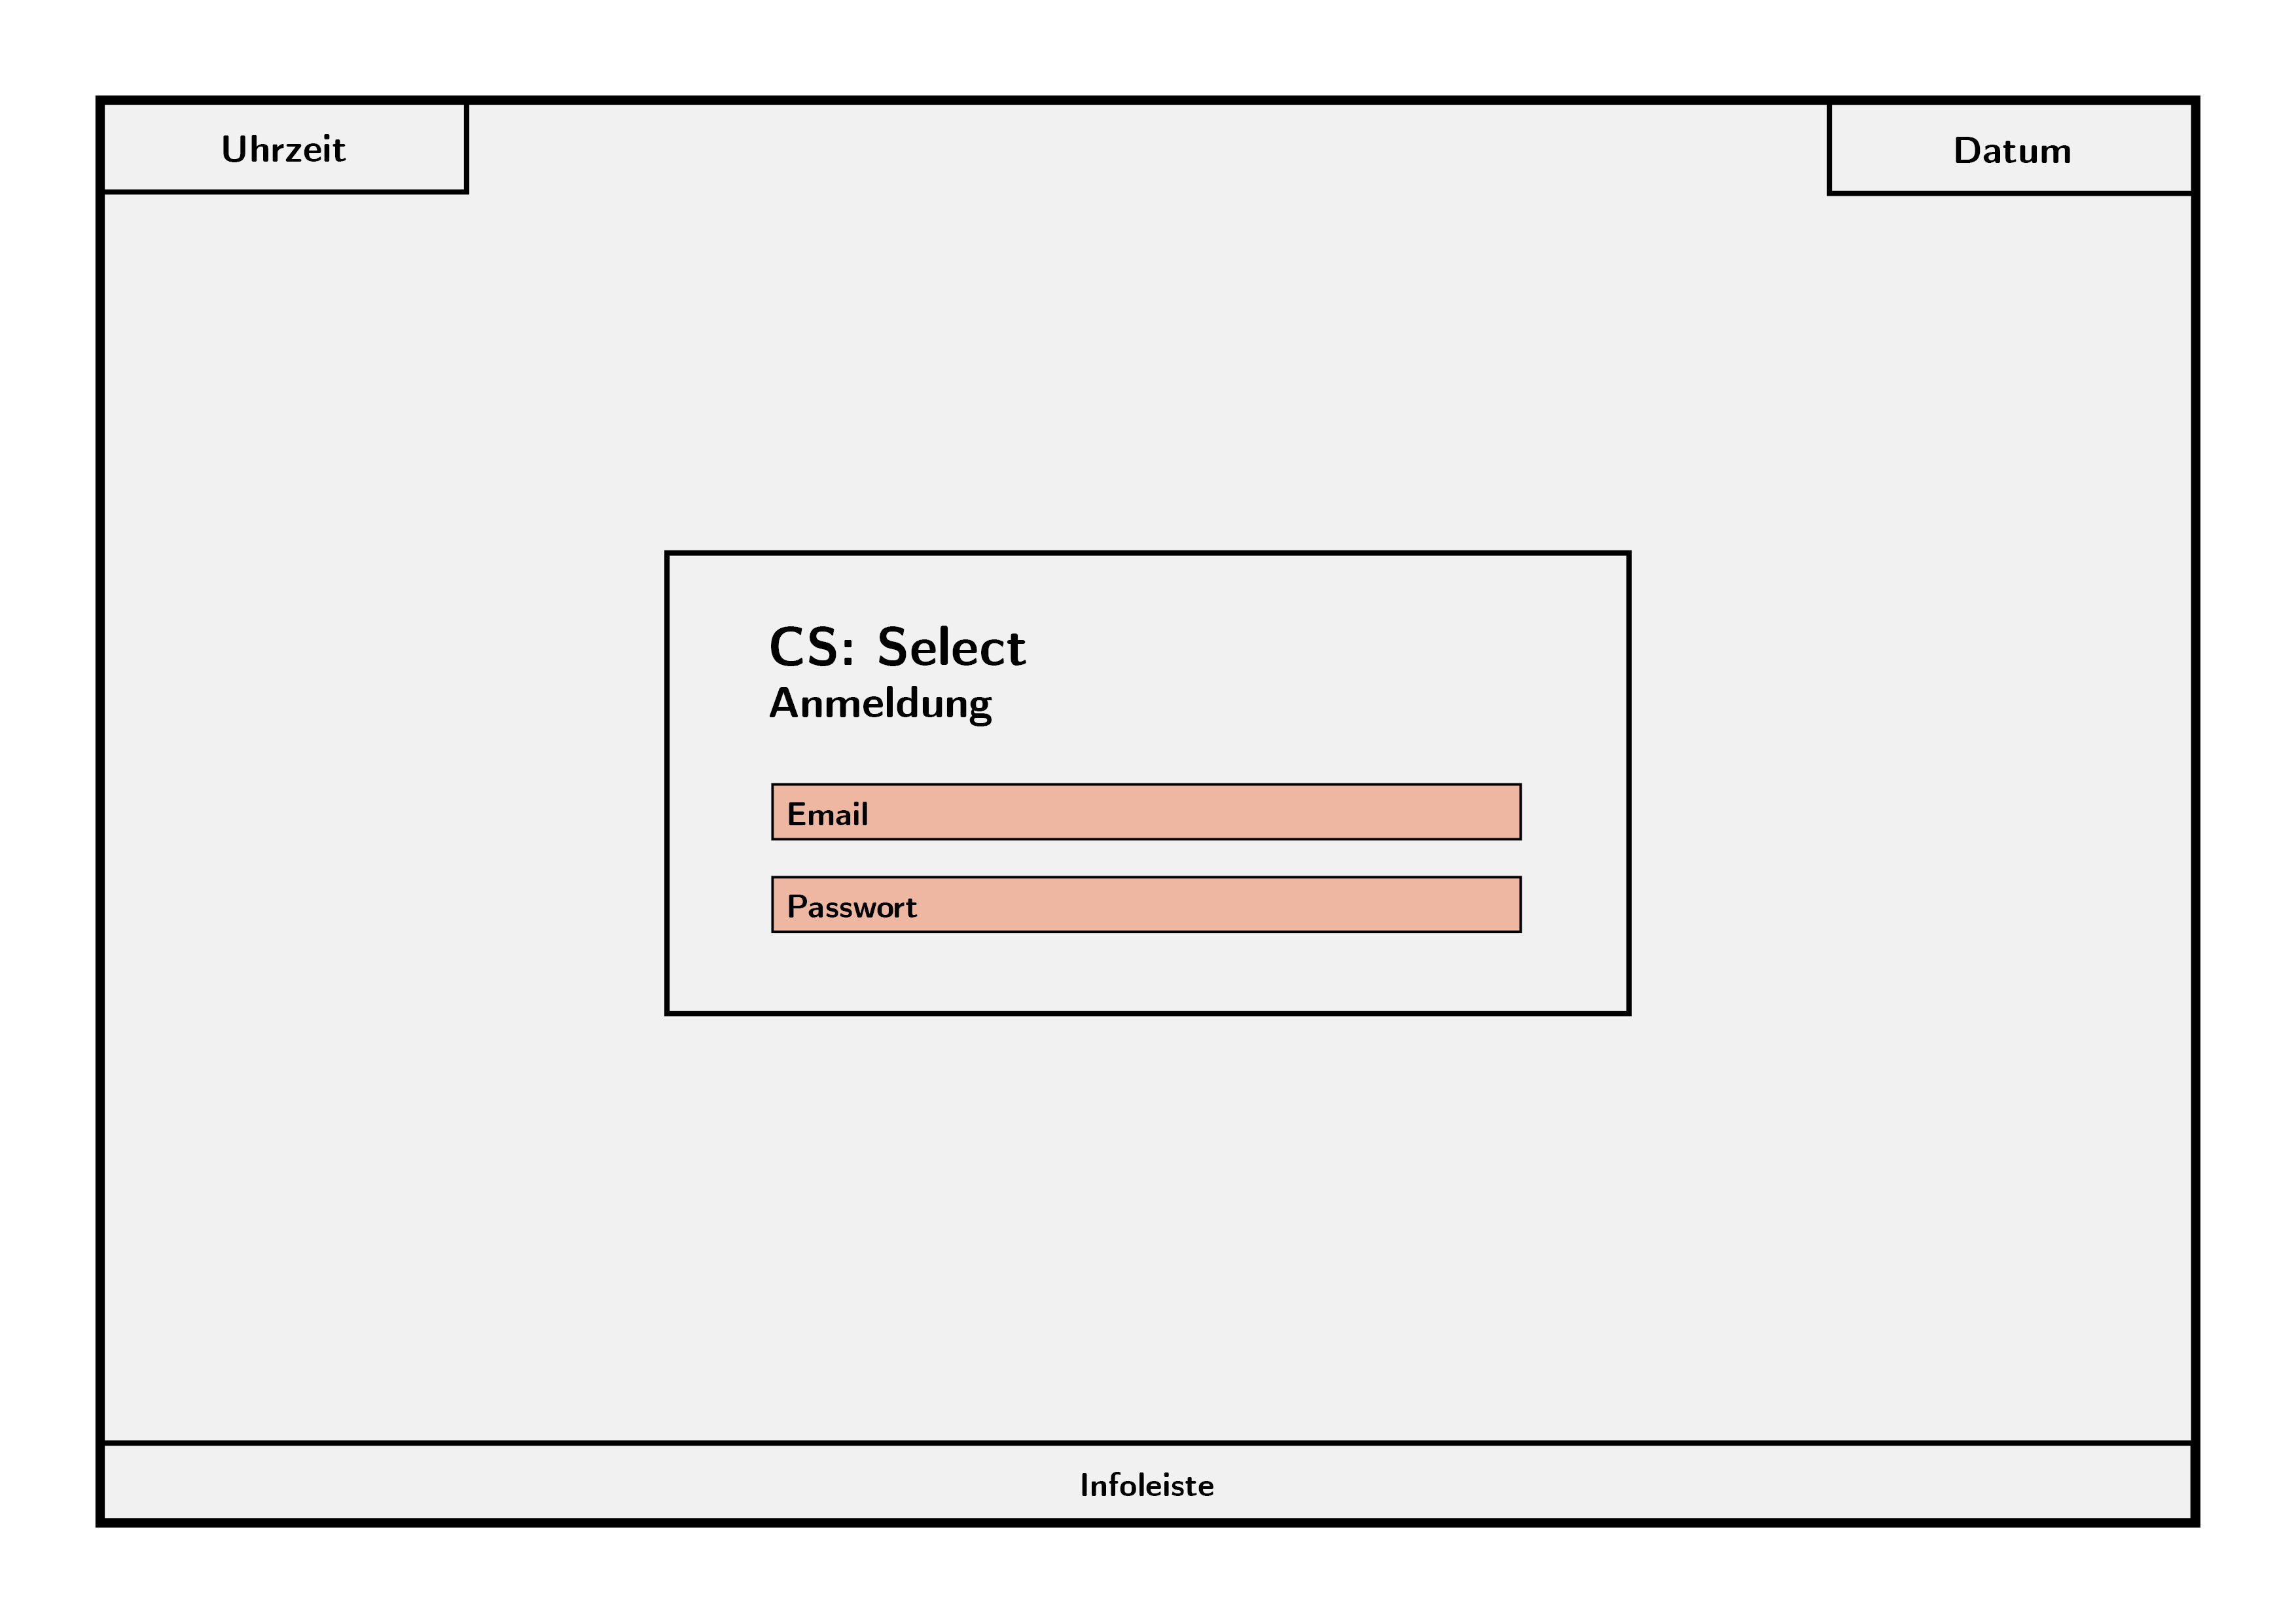
\includegraphics[width=400px]{../pictures/1_Anmeldung.jpg}
    \subsection{Organisator-Start (Desktop)}
    \centering
    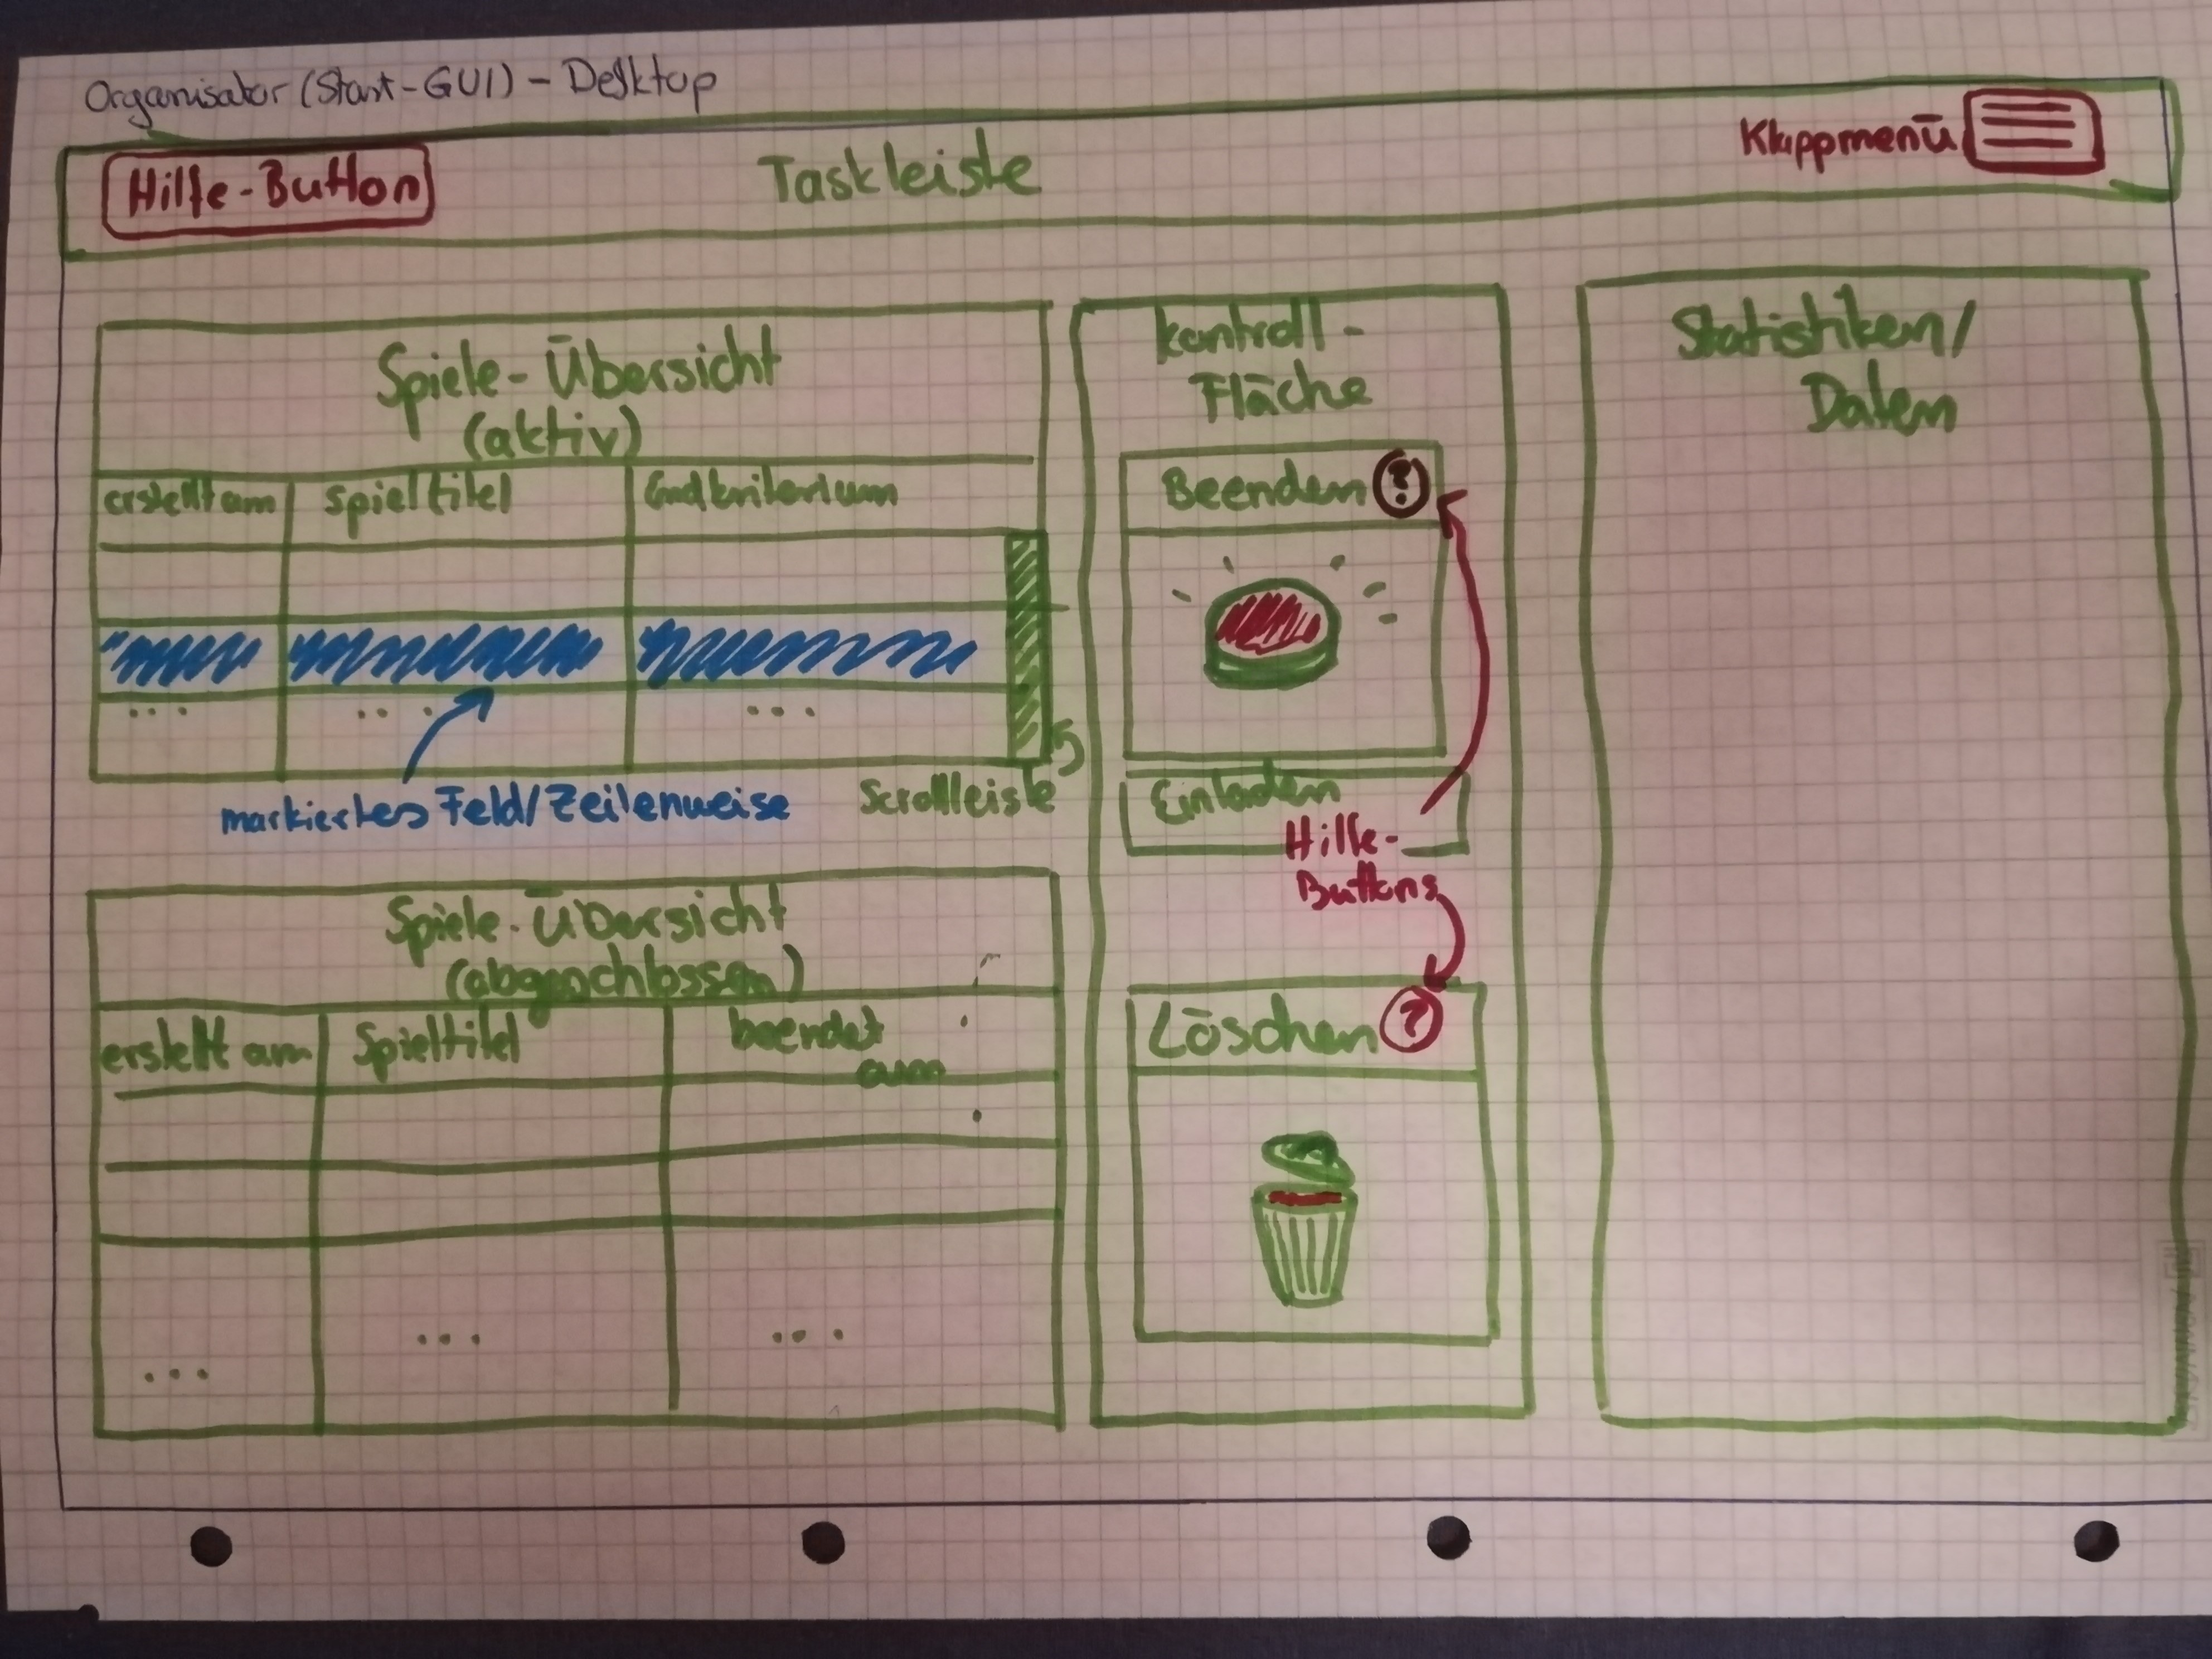
\includegraphics[width=400px]{../pictures/2_Organisator.jpg}
    \subsection{Organisator-Start (Responsive)}
    \centering
    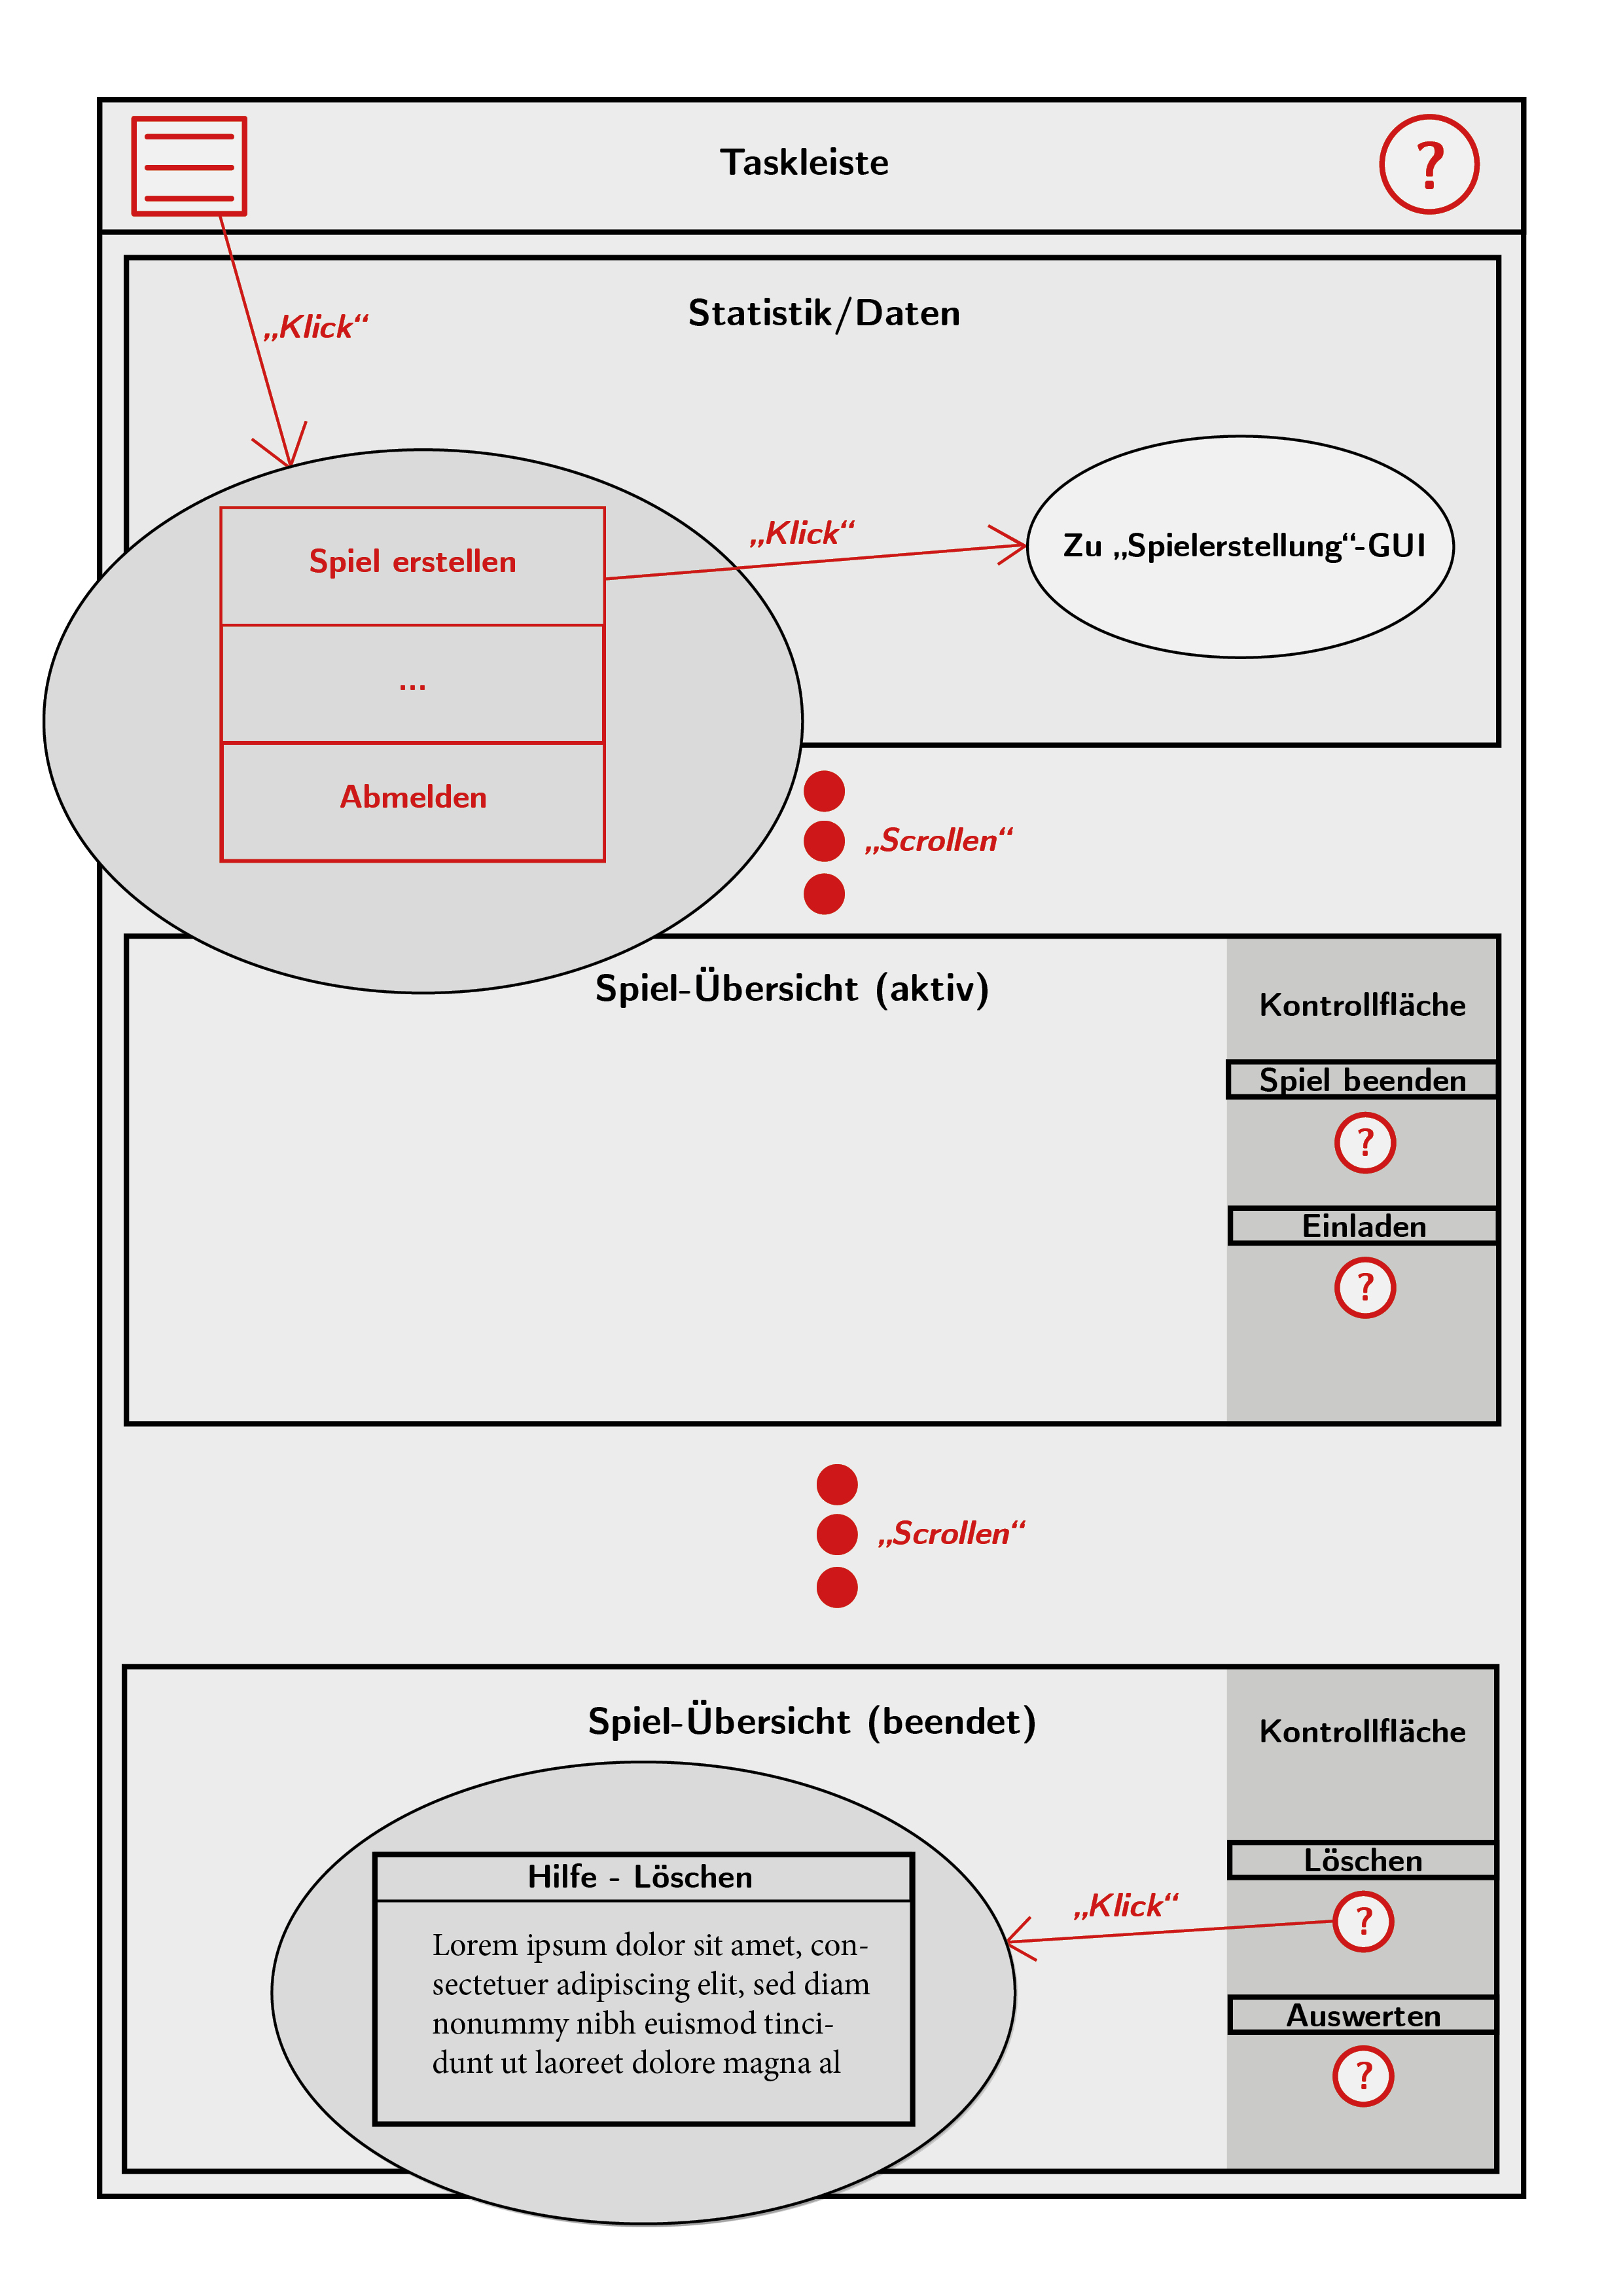
\includegraphics[width=400px]{../pictures/3_Organisator(responsive).jpg}
    \subsection{Spielerstellung}
    \centering
    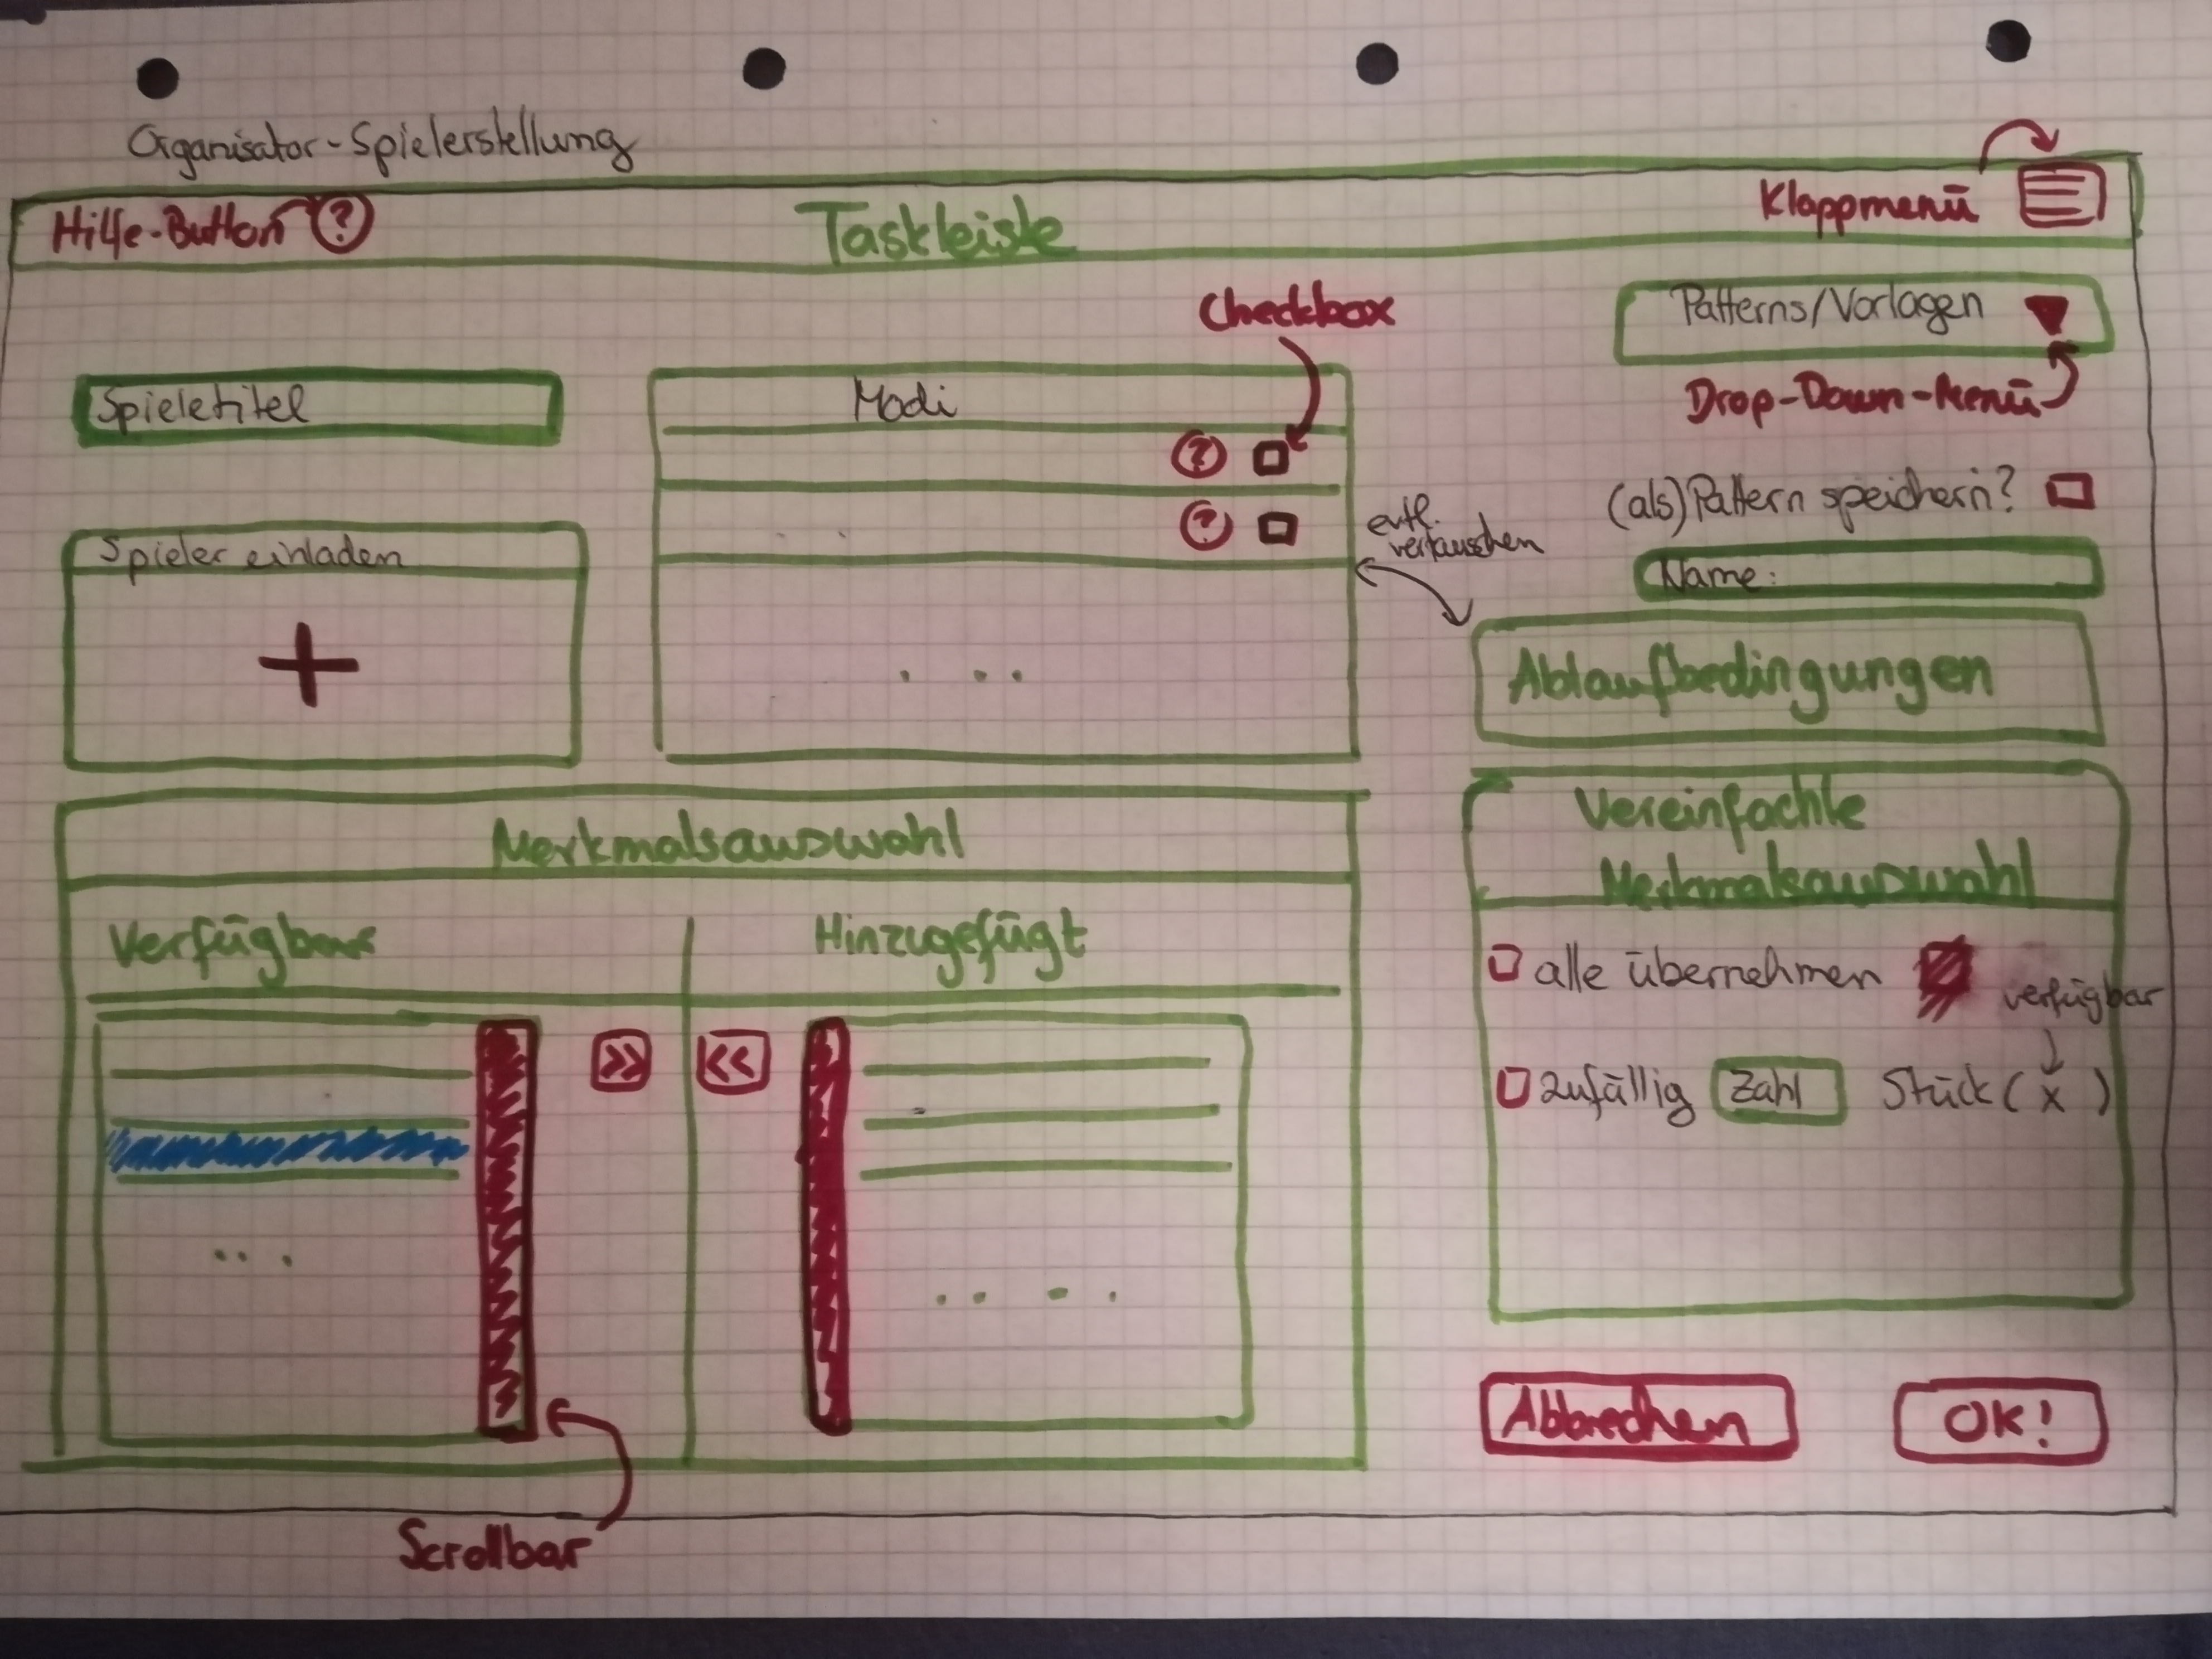
\includegraphics[width=400px]{../pictures/4_Spielerstellung.jpg}
    \subsection{Spieler-Übersicht}
    \label{fig:Spieler-Übersicht}
    \centering
    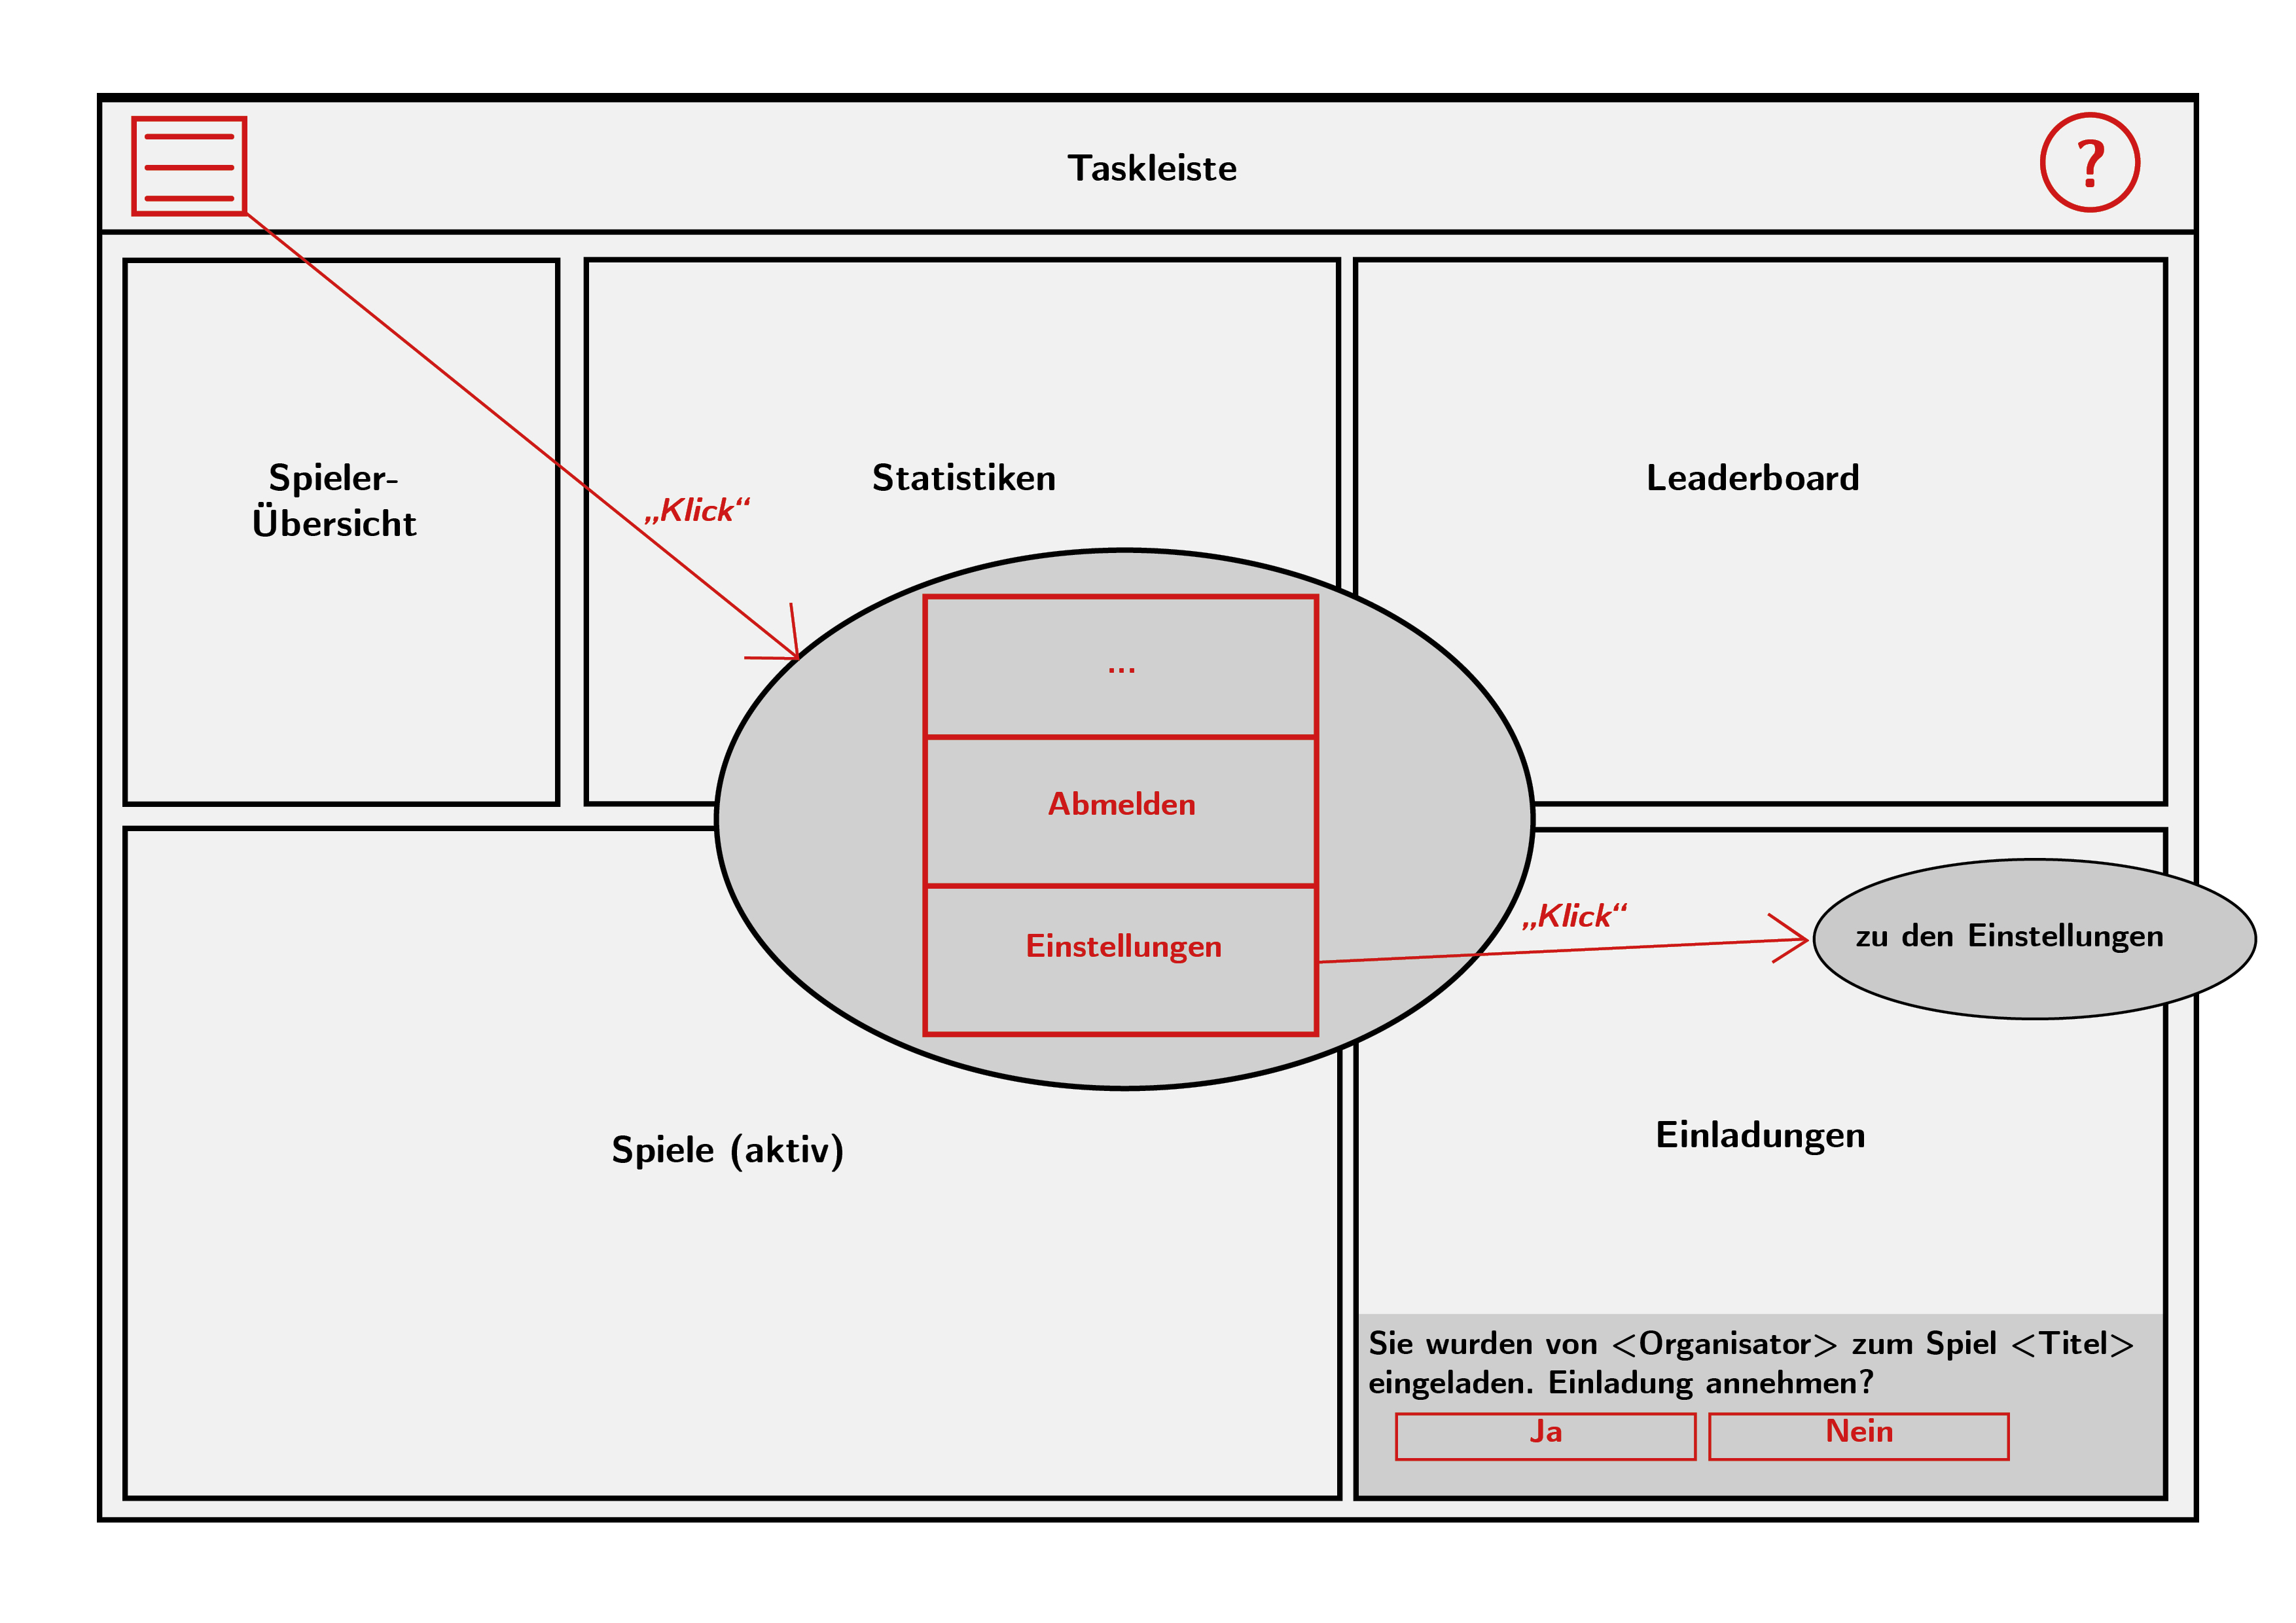
\includegraphics[width=400px]{../pictures/5_Spieler.jpg}
    \subsection{Spiel}
    \centering
    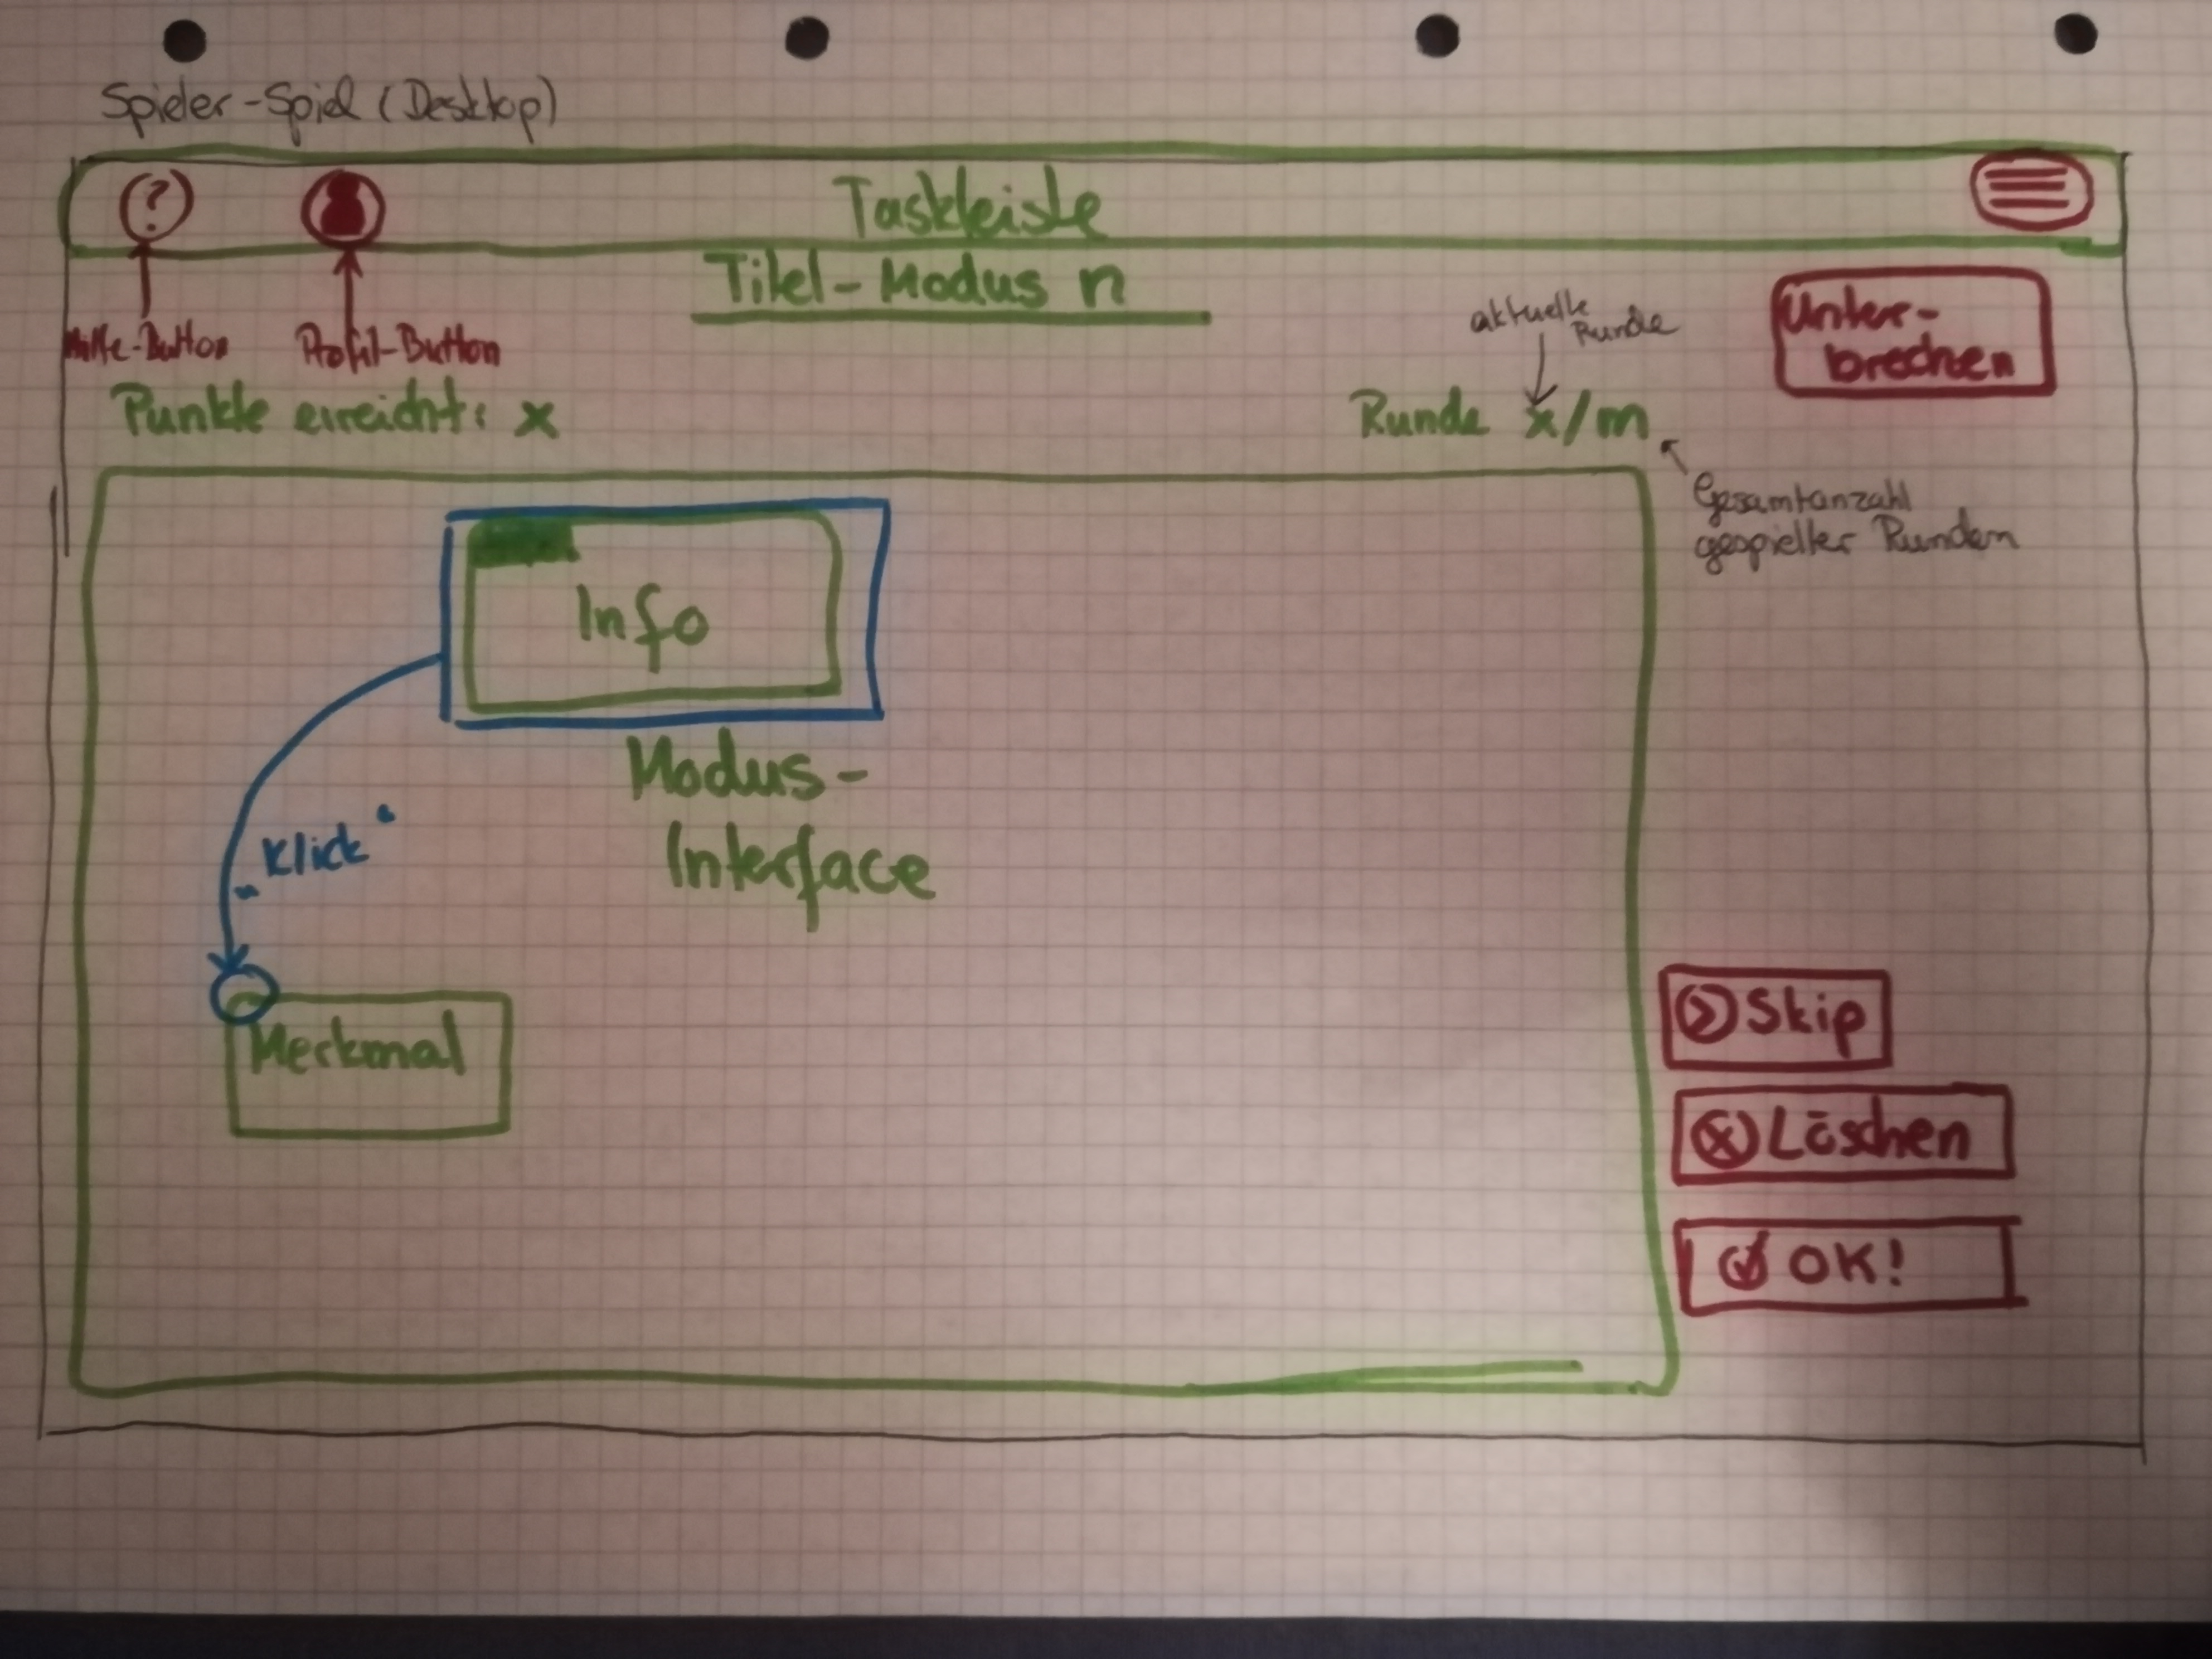
\includegraphics[width=400px]{../pictures/6_Spiel.jpg}
    \clearpage
    \chapter{Glossar}
    \printglossary[title=Glossar]
\end{document}
